\documentclass{TDP005mall}
\usepackage{graphicx}
\usepackage{float}


\newcommand{\version}{Version 1.1}
\author{Martin Kuiper, \url{marku849@student.liu.se}\\
  Jim Teräväinen, \url{jimte145@student.liu.se}}
\title{Designspecifikation}
\date{\today}
\rhead{Martin Kuiper\\
Jim Teräväinen}



\begin{document}
\projectpage
\section{Revisionshistorik}
\begin{table}[!h]
\begin{tabularx}{\linewidth}{|l|X|l|}
\hline
Ver. & Revisionsbeskrivning & Datum \\\hline
1.1 & Ändringar i UML diagram, tick blev update på många ställen och vissa publika variabler blev private & 2020-12-03 \\\hline
1.0 & Första utkast för designspecifikationen. & 2020-11-27 \\\hline
\end{tabularx}
\end{table}


\begin{figure}[H]
         \begin{center}
             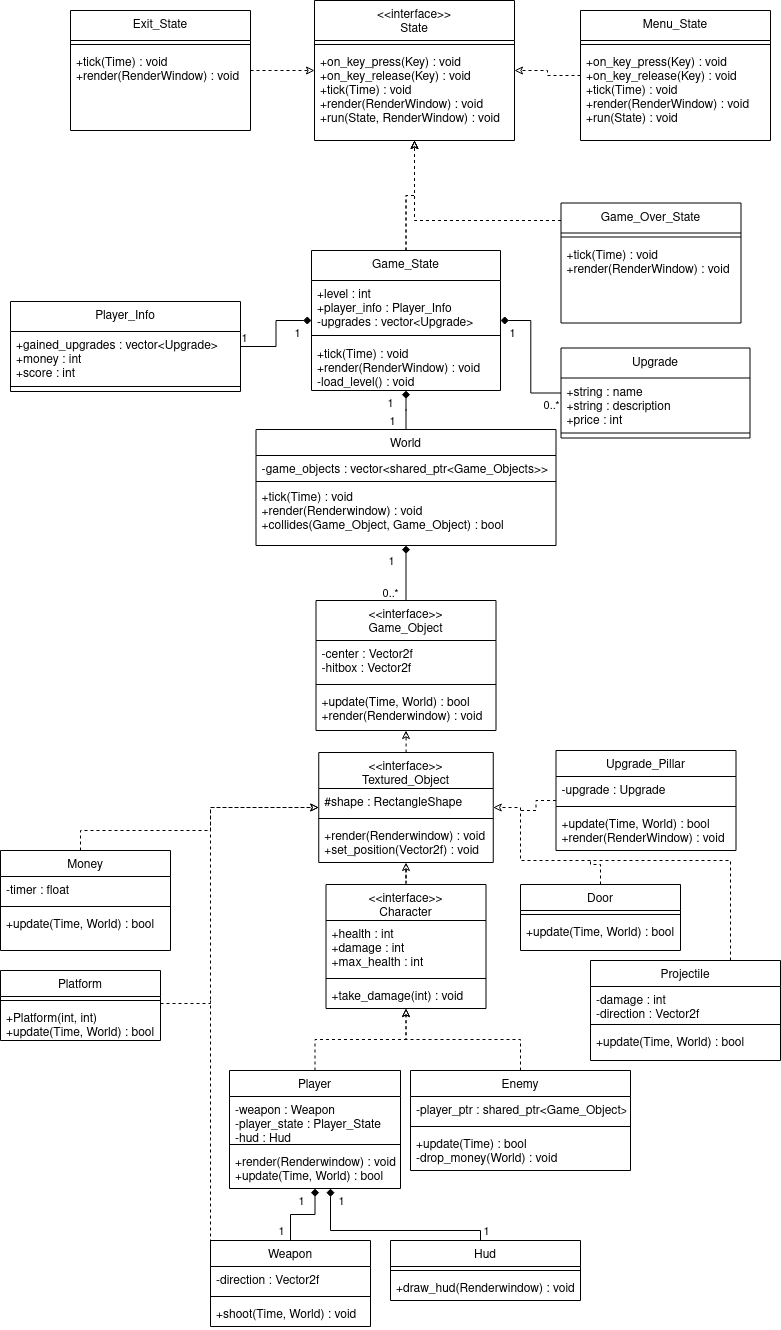
\includegraphics[width=15cm]{Graphic/overview.png}
             \caption{\label{fig:1} Övergripande UML diagram för strukturen i spelet.}
         \end{center}
\end{figure}

\section{Beskrivning av övergripande system}

\subsection{Stadier}
Grunden för spelet ligger i att vi skapar olika stadier som sedan körs och hanterar underfunktioner. Dessa stadier representeras i toppen av figur \ref{fig:1} med namn som innehåller 'state'. När spelet startar skapas ett 'Menu\_State' där spelaren kan välja mellan olika alternativ. Alternativen leder till olika saker men oftast till att vi startar spelet igenom att köra vårt 'Game\_State'. 

'Game\_State' kommer att existera under hela körtiden och håller därför koll på viss information som vi behöver behålla. Detta inkluderar saker som hur många spelplaner spelaren klarat (level) för att skala upp svårighetsgraden. Det håller även koll på viss information som behöver vara konstant när vi skapar om spelaren för varje spelplan som hur mycket pengar och vilka uppgraderingar spelaren har. Allting under 'Game\_State' kommer att försvinna och skapas igen på nya platser för varje spelplan vi laddar in.

\subsection{Världen och objekt}
Världen representeras av klassen 'World' och hanterar ett obestämt antal 'Game\_Object' som alla har en position och 'hitbox'. Dessa objekt bildar tillsammans det komplexa system som är spelet. Alla objekt har en textur och ärver därmed från klassen 'Textured\_Object' som kommer hjälpa till att hantera texturerna för objekten. Klassen Game\_State har hand om att skapa och hålla koll på finderna som ska dyka upp på spelplanen. Så länge som rätt mängd fiender för nuvarande 'level' inte skapats så kommer den fortsätta att skapa fiender med ett visst tidsintervall, detta också baserat på 'level'.

Klassen 'Character' ärver från 'Textured\_Object' och innehåller allt som spelare och fiender har gemensamt, som att de har hälsa och skada. Hälsa representerar hur mycket skada en karaktär kan ta innan den raderas från spelplanen, och i spelarens fall förlorar. Hälsa är individuellt och sparas i alla objekt för sig, det går ned när objektet tar skada. Skada representerar hur mycket hälsa spelaren eller en fiende förlorar när de blir nuddade av något som gör skada.

'Player' representerar spelarkaraktären och hanterar sin rörelse, hur den reagerar på kollisioner, och sitt 'Weapon'. 'Player' kan tillkalla funktionen 'shoot()' i sitt weapon så att det avfyras en projektil i vapnets riktning. Denna projektil ärver sin skada från spelaren så att vi enkelt kan modifiera skadan en spelares projektil gör med uppgraderingar och liknande.

'Enemy' hanterar sin egen rörelse och rör sig mot spelaren för att skada denna.

\subsection{Objekt med få funktioner}
'Money' har helt enkelt ett värde som läggs till på spelarens pengar när de kolliderar med dem. Vi valde av tematiska skäl att visa pengarna som Själar för spelaren men funktionen är oförändrad. 

'Hud' ritar ut hur mycket hälsa och pengar spelaren har så att spelaren enkelt kan se om de är påväg att förlora eller har råd med en uppgradering. 

'Platform' hanterar de plattformar som spelaren kan stå på i nivån utöver botten av skärmen. 

'Door' skapas på kordinater enligt 'load\_level()' när alla fiender besegrats. Genom att interagera med dörren laddas nästa spelplan in. 

'Upgrade\_Pillar' skapas också enligt koordinater från 'load\_level()' när alla fiender besegrats och innehåller en slumpad uppgradering. Denna uppgradering kan läggas till i 'player\_info' om spelaren har nog med pengar (själar) för att köpa den och väljer att gör det.

\section{Klassbeskrivningar}
\subsection{Player}
Player ska kunna uppdatera sin position beroende på vilka knappar som är intryckta samt vilket state Player har.
Player har en överlagrad render()-funktion, då den behöver kunna uppdatera hur den renderas beroende på vad som händer Player-objektet.
Funktionen update() kallar alla funktioner som ska köra när spelet uppdateras. 

\subsubsection{Viktiga datamedlemmar}
\begin{itemize}
\item state - påverkar hur objektet beter sig när update() kallas.
\item weapon - ett objekt av klassen Weapon ägs av Player.
\item hud - ett objekt av klassen Hud ägs av Player.
\item activate\_popup - ett textobjekt som visas när spelaren kan interagera med vissa andra objekt.
\item player\_info - en referens till Player\_Info-objektet som håller reda på saker som spelarens insamlade score och pengar.
\item invincible - hur länge Player ska vara osårbar.
\item max\_jumps - hur många gånger Player kan hoppa utan att nudda marken.
\item health - ärvd från Character, minskar när Player tar skada.
\item damage - ärvd från Character, påverkar Players vapens skada.
\item speed - ärvd från Character, påverkar hastigheten av objektets förflyttning.
\item shape - ärvd från Textured\_Object, påverkar hur objektets textur ritas ut.
\item center - ärvd från Game\_Object, bestämmer objektets position på skärmen.
\item hitbox - ärvd från Game\_Object, bestämmer storleken på objektets kollisionsområde.
\end{itemize}

\subsubsection{update(Time)}
Vid varje uppdatering av spelet kallas Players update-funktion av det ägande World-objektet. Funktionen har i uppdrag att utföra följande:

För att flytta Player kallas move\_player().

För att flytta och skjuta vapnet kallas handle\_weapon().

För att hantera Players kollisionsbeteende med andra objekt kallas handle\_collision().

För att hantera animationerna av Players textur kallas handle\_animation().

Datamedlemmen 'invincible' minskas med tiden som passerat sen den senaste uppdateringen om den inte är 0.

Det ägda Hud-objektets datamedlemmar uppdateras så att nuvarande hälsa, pengar och poäng visas på skärmen. 

En datamedlem i Player\_Info uppdateras så att Game\_State vet om spelaren har dött eller inte.

Slutligen returneras spelarens levandestatus till World så att den inte tas bort om den inte är död.

\subsubsection{move\_player()}
För att hantera den horisontella rörelsen kallas funktionen handle\_horizontal\_move().
Den flyttar karaktären beroende på vilka tangenter som är intryckta.

För att hantera hopp-input kallas handle\_jump\_input().
Den ser till att när spelaren trycker på hopp-knappen ändras state till 'jumping' om spelaren inte redan hoppat maximalt antal gånger utan att landa. 

För att kolla om spelaren ska börja falla från en platform kallas funktionen handle\_drop().

Om player\_state är satt till 'jumping' kallas jump() för att hantera hopp-rörelsen.
Efter en viss tid sätter jump() player\_state till 'falling'.

Om player\_state är satt till 'falling' kallas fall() för att hantera fall-rörelsen.

Normalt är player\_state satt till 'standing'. 


\subsubsection{handle\_weapon()}
Players position bestämmer Weapon-objektets position. 

Input från tangentbord eller muspekare bestämmer vapnets rotation.
Vapnet har en datamedlem 'fire\_rate' som påverkar hur ofta det kan avfyras. 

Är 'Avfyra vapen'-knappen intryckt och vapnets 'fire\_rate' 0 skapas en projektil.
Projektilen rör sig i riktningen av vapnets rotation och har en datamedlem 'damage' som sätts till Players 'damage'.

\subsubsection{handle\_collision(World)}
Player frågar World vilka objekt den kolliderar med. Kolliderar Player med ett Enemy-objekt kallas take\_damage().


Om den understa delen av Player-objektet kolliderar med den översta delen av en plattform sätts 'falling' till 'standing'.


\subsubsection{take\_damage(int)}
Players 'health' subtraheras med skadan som skickas som parameter till funktionen. 

Datamedlemmen 'immune' sätts enligt hur länge Player ska vara odödlig efter att ha tagit skada.


\subsection{Hud}
HUD står för Heads-Up Display och har som syfte att visa relevant information för spelaren. 
Hud-klassen ska visa Player-objektets nuvarande hälsa (health) samt spelarens insamlade pengar.

\subsubsection{Datamedlemmar}
\begin{itemize}
\item player\_ptr - pekare till player för att kunna hämta dess hälsa.
\item shape - ärvd från Textured Object, påverkar hur objektets textur ritas ut.
\item center - ärvd från Game\_Object, bestämmer objektets position på skärmen.
\item hitbox - ärvd från Game\_Object, bestämmer storleken på objektets kollisionsområde.
\end{itemize}

\subsubsection{tick(Time)}
Player-objektets hälsa hämtas och en grafik med den informationen ritas ut i kanten av skärmen ovanpå alla andra objekt.

Mängden insamlade pengar hämtas från Game\_States datamedlem player\_info och renderar detta på liknande sätt. 


\section{Designens för- och nack-delar}
Vi har försökt hålla designen så simpel som möjligt genom att designa klasser som ärver så mycket funktion som möjligt. I vissa fall kan detta spara oss mycket jobb då våra klasser inte kräver så lång kod. Nackdelen med detta är att vi har mycket beroende av föräldrar i alla våra klasser och får svårt att skapa mer nischat beteende. Vi har tänkt mycket på hur vi ska komma runt problem som vi skapat för oss själva igenom arvet och kommit fram till strukturen som vi har nu. Systemet med att olika states för att hantera vad spelet ska göra just nu verkar väldigt smidigt och gör det enkelt att hantera saker som menyer och att stänga av spelet. Det hade självklart varit enklare att skriva en spel-loop i huvudfunktionen men i slutändan kommer detta att spara oss mycket tid i form av mindre omstrukturering när vi vill lägga till en meny för exempelvis inställningar.

Ett exempel på hur arvet i vår design kan bli problematiskt är när 'spawner' behöver en position och bör ägas av 'world'. Det passar väldigt bra att 'spawner' är ett 'Game\_Object men det leder till att vi inkluderar en onödig men ofarlig funktion i form av en 'hitbox'. En 'spawner' behöver ingen hitbox då den aldrig ska interagera med spelaren, fiender eller något annat på spelplanen, men samtidigt skadar det inte så det var värt det enligt oss att göra på det här sättet. Om vi inte är försikta eller förbereder oss på det så kan det dock lätt bli att vi implementerar beteende som ska påverka alla objekt med en 'hitbox' och inte tänker på att 'spawner' har en. Detta bör undersökas hur det går att skydda mot som, exempelvis genom att göra 'spawner's 'hitbox' oåtkomlig av andra funktioner.

En annan lösning på detta skulle vara att flytta egenskapen att ha en 'hitbox' till de objekt som ärver av 'Textured\_Object'. Detta skulle dock inte heller vara bra då 'Hud' inte heller behöver en hitbox men fortfarande hade fått en. Att skapa flera klasser för att lösa problemet är inte heller fördelaktigt då 'Spawner' inte ska synas och 'Hud' ska det, därmed kan de inte dela en klass för objekt som inte ska ha en 'hitbox'. Den lösningen som är implementerad just nu anser vi vara den bättre.

\section{Externa filformat} 
Funktionen 'load\_level()' i 'World' kommer att använda en textfil av något slag med ett par olika definerade nivåer. Planen är att använda ren text med olika ikoner eller en json-fil med kordinater för placering av plattformar, spelare, uppgraderingsstationer och avslutningsdörr. Med detta så ska man enkelt kunna definera upp nya nivåer igenom att lägga till data i filen som tolkas av vår funktion för att ladda spelplanen. Mest användarvänligt hade varit att låta användaren rita upp spelplanen med olika tecken som representerar olika objekt som kan placeras ut. Detta skulle även automatiskt lösa risken att man placerar något på samma plats då textfiler inte godkänner flera tecken på samma plats.

Alternativet skulle vara att låta användaren beskriva spelplanen med hjälp av ord och siffror i en json-fil. Detta sätt blir lättare att implementera för oss men ger inte samma tilltalande gränssnitt att skapa i. Det är lättare för användaren att faktiskt rita upp en spelplan med text än att visualisera planen medan den skriver upp siffror.

\end{document}
